\documentclass[12pt,a4paper]{article}

% --- Packages ---
\usepackage[utf8]{inputenc}
\usepackage{amsmath,amssymb,amsfonts}
\usepackage{physics}
\usepackage{siunitx}
\usepackage{hyperref}
\usepackage{geometry}
\usepackage{tcolorbox}
\usepackage{booktabs}
\usepackage{graphicx}
\usepackage{pgfplots} % For self-contained plotting
\pgfplotsset{compat=1.17}

\geometry{margin=1in}

% --- Custom Colors for Links ---
\hypersetup{
    colorlinks=true,
    linkcolor=blue,
    urlcolor=cyan,
}

\title{Provisional Derivations for the Ware Constant $W$: Informational Flux and Action Principle}
\author{William B. Ware}
\date{December 2025}

\begin{document}

\maketitle

\begin{tcolorbox}[colback=yellow!5!white,colframe=yellow!50!black,title=Cautionary Note]
The contents of this document are \textbf{provisional and phenomenological}. These derivations serve as placeholders to ensure mathematical consistency while the first-principles derivation from the Primordial Informational Field (PIF) is finalized. For the established foundation, see the \href{https://github.com/YourRepo/Core_Derivations.pdf}{Core Derivations Paper}.
\end{tcolorbox}

\begin{abstract}
This document records elements of the Ware Constant framework that are mathematically consistent and empirically motivated, but not yet uniquely derived from a fundamental action principle. We outline a Scalar-Vector-Tensor (SVT) hybrid Lagrangian, the resulting $1/r$ acceleration law, and the schematic form of the Informational Flux Tensor.
\end{abstract}

\section{Informational Acceleration Law}

The total acceleration experienced by a test body is modeled as the sum of the Newtonian and Informational components:
\begin{equation}
\mathbf{a}_{\rm total} = \mathbf{a}_{\rm N} + \mathbf{a}_{\rm info} = -\frac{GM}{r^2}\hat{\mathbf{r}} + W \frac{G M}{r_0\, r} \hat{\mathbf{r}} \label{eq:atotal}
\end{equation}

\noindent This formulation ensures a transition to flat rotation curves. The transition radius $r_{\rm trans}$, where the informational acceleration equals the Newtonian pull ($|\mathbf{a}_{\rm N}| = |\mathbf{a}_{\rm info}|$), is given by:
\begin{equation}
r_{\rm trans} = \frac{r_0}{W} \label{eq:rtrans}
\end{equation}

% --- Self-Contained Figure ---
\begin{figure}[h!]
    \centering
    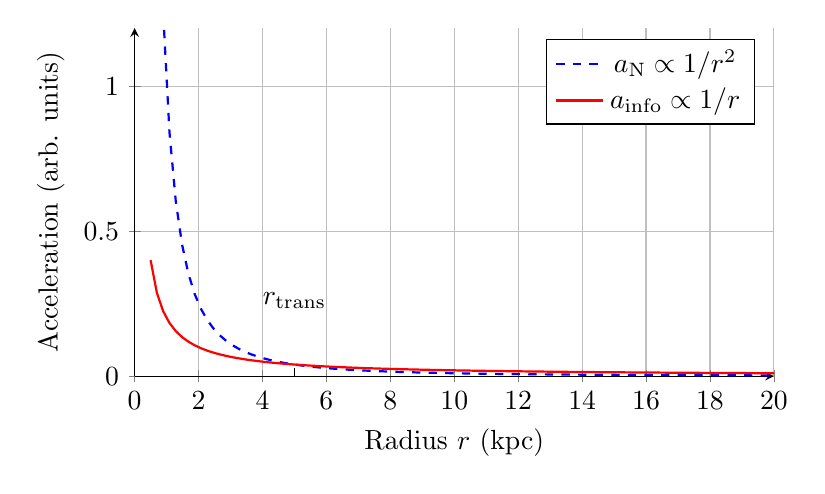
\begin{tikzpicture}
    \begin{axis}[
        width=0.8\textwidth,
        height=6cm,
        xlabel={Radius $r$ (kpc)},
        ylabel={Acceleration (arb. units)},
        xmin=0, xmax=20,
        ymin=0, ymax=1.2,
        domain=0.5:20,
        samples=100,
        axis lines=left,
        legend pos=north east,
        grid=major
    ]
        % Newtonian 1/r^2
        \addplot[blue, thick, dashed] {1/x^2};
        \addlegendentry{$a_{\rm N} \propto 1/r^2$}
        
        % Ware 1/r (scaled slightly for visibility)
        \addplot[red, thick] {0.2/x}; 
        \addlegendentry{$a_{\rm info} \propto 1/r$}
        
        % Transition point marker
        \draw[dashed, black] (axis cs:5,0) -- (axis cs:5,0.04);
        \node[above] at (axis cs:5, 0.2) {$r_{\rm trans}$};
    \end{axis}
    \end{tikzpicture}
    \caption{Schematic transition from Newtonian dominance ($r < r_{\rm trans}$) to Informational dominance ($r > r_{\rm trans}$). The crossover point is defined by $r_{\rm trans} = r_0/W$.}
    \label{fig:transition}
\end{figure}

\section{Parameter Definitions}

To ensure consistency in numerical simulations (e.g., Python/SciPy rotation curve scripts), the following parameter definitions are adopted.

\begin{table}[h!]
\centering
\begin{tabular}{@{}llll@{}}
\toprule
\textbf{Symbol} & \textbf{Value / Relation} & \textbf{Units} & \textbf{Description} \\ \midrule
$W$ & $\approx 0.08$ & [1] & Dimensionless coupling constant \\
$r_0$ & $\sim 1 \text{ kpc}$ & [L] & Coherence length ($\propto \rho_{\rm info}^{-1/2}$) \\
$r_{\rm trans}$ & $r_0 / W \approx 12.5 \text{ kpc}$ & [L] & Transition radius \\
$\rho_{\rm info}$ & Microphysical variable & [L$^{-4}$] & Informational density of vacuum \\ 
\bottomrule
\end{tabular}
\caption{Provisional parameters for the Ware framework.}
\label{tab:params}
\end{table}

\section{Provisional Informational Lagrangian (SVT Hybrid)}

To formalize the physics, we introduce a provisional Scalar-Vector-Tensor (SVT) Lagrangian. This structure is architecturally similar to TeVeS or MoG frameworks but driven by informational density:
\begin{equation}
\mathcal{L}_{\rm info} = -\frac{1}{4} F_{\mu\nu}^{\rm info} F^{{\rm info}\,\mu\nu} + J_\mu^{\rm info} A_{\rm info}^\mu + \mathcal{V}(\phi_{\rm info}) \label{eq:lagrangian}
\end{equation}

\noindent The total action integrates these degrees of freedom with the Einstein-Hilbert action:
\begin{equation}
S_{\rm total} = \int d^4x \sqrt{-g} \Big[ \frac{1}{16\pi G} R + \mathcal{L}_{\rm matter} + W\, \mathcal{L}_{\rm info} \Big] \label{eq:action}
\end{equation}

\section{Informational Flux Tensor Form}

For numerical implementation in GR solvers, the Informational Flux Tensor $T_{\mu\nu}^{\rm info}$ is derived from Eq. \ref{eq:lagrangian}. Neglecting the scalar potential for the kinetic limit, it takes the Maxwell-like form:

\begin{equation}
T_{\mu\nu}^{\rm info} = F_{\mu\lambda}^{\rm info}F^{\lambda}_{\nu} - \frac{1}{4}g_{\mu\nu}F^{\alpha\beta}_{\rm info}F_{\alpha\beta}^{\rm info}
\end{equation}

\noindent \textbf{Implementation Note:} Unlike standard electromagnetism, this tensor couples to the metric with strength $W$. In a static, spherically symmetric spacetime, the $T_{00}^{\rm info}$ component represents the energy density responsible for the effective "dark halo" potential.

\section{Notes for Collaborators}
\begin{itemize}
    \item \textbf{Field Categorization:} This is an SVT hybrid. $A_\mu^{\rm info}$ provides vector-led directionality (flux), while $\phi_{\rm info}$ handles the scaling of $r_0$.
    \item \textbf{Theoretical Frontier:} A primary goal is to derive $W$ and $r_0$ directly from the entropy-gradient of the PIF.
    \item \textbf{Validation:} See \href{https://github.com/YourRepo/Stability_Analysis.pdf}{Stability Analysis} for preliminary ghost-free condition checks.
\end{itemize}

\end{document}
